% Richiede: \usepackage{pgfplots} \pgfplotsset{compat=1.18}
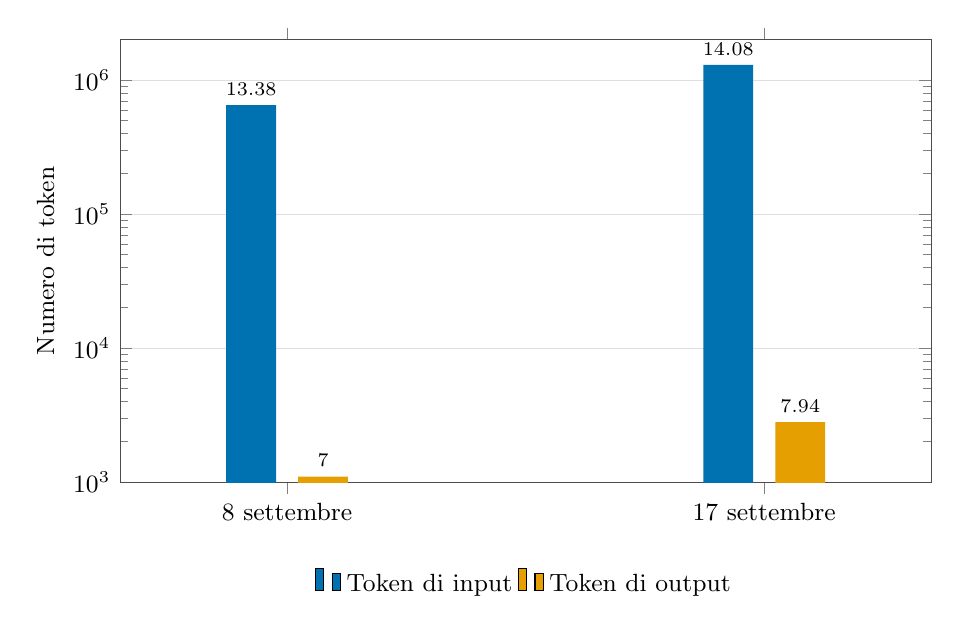
\begin{tikzpicture}
\definecolor{poliblue}{HTML}{0072B2}
\definecolor{poliorange}{HTML}{E69F00}
\begin{semilogyaxis}[
  width=0.98\linewidth,
  height=7.2cm,
  ymin=1000,
  ymax=2000000,
  ylabel={Numero di token},
  symbolic x coords={8 settembre,17 settembre},
  xtick=data,
  ymajorgrids=true,
  grid style={gray!25},
  axis line style={black!70},
  tick label style={font=\small},
  label style={font=\small},
  legend style={at={(0.5,-0.18)},anchor=north,legend columns=2,draw=none,font=\small},
  ybar=8pt,
  bar width=18pt,
  enlarge x limits=0.35,
]
\addplot[fill=poliblue,draw=none,nodes near coords,every node near coord/.append style={font=\scriptsize}]
  coordinates {(8 settembre,650000) (17 settembre,1300000)};
\addplot[fill=poliorange,draw=none,nodes near coords,every node near coord/.append style={font=\scriptsize}]
  coordinates {(8 settembre,1100) (17 settembre,2800)};
\legend{Token di input,Token di output}
\end{semilogyaxis}
\end{tikzpicture}

